\chapter{Interpreter模式}
\section{解释器模式的概念}
\section{定义}
解释器(Interpreter)模式的定义:给分析对象定义一个语言,并定义该语言的文法表示,再设计一个解析器来解释语言中的句子。也就是说,用编译语言的方式来分析应用中的实例。这种模式实现了文法表达式处理的接口,该接口解释一个特定的上下文。
\section{优点}
\begin{enumerate}
	\item 扩展性好。由于在解释器模式中使用类来表示语言的文法规则,因此可以通过继承等机制来改变或扩展文法。
	\item 容易实现。在语法树中的每个表达式节点类都是相似的,所以实现其文法较为容易。
\end{enumerate}
\section{缺点}
\begin{enumerate}
	\item 执行效率较低。解释器模式中通常使用大量的循环和递归调用,当要解释的句子较复杂时,其运行速度很慢,且代码的调试过程也比较麻烦。
	\item 会引起类膨胀。解释器模式中的每条规则至少需要定义一个类,当包含的文法规则很多时,类的个数将急剧增加,导致系统难以管理与维护。
	\item 可应用的场景比较少。在软件开发中,需要定义语言文法的应用实例非常少,所以这种模式很少被使用到。
\end{enumerate}
\section{解释器模式的角色}
\begin{enumerate}
	\item AbstractExpression抽象表达式:定义解释器的接口,约定解释器的解释操作,主要包含解释方法 interpret()。
	\item TerminalExpression终结符表达式:是抽象表达式的子类,用来实现文法中与终结符相关的操作,文法中的每一个终结符都有一个具体终结表达式与之相对应。
	\item NonterminalExpression非终结符表达式:是抽象表达式的子类,用来实现文法中与非终结符相关的操作,文法中的每条规则都对应于一个非终结符表达式。
	\item Context上下文:通常包含各个解释器需要的数据或是公共的功能,一般用来传递被所有解释器共享的数据,后面的解释器可以从这里获取这些值。
	\item Client请求者:主要任务是将需要分析的句子或表达式转换成使用解释器对象描述的抽象语法树,然后调用解释器的解释方法,当然也可以通过环境角色间接访问解释器的解释方法。
\end{enumerate}
\section{应用场景}
\begin{enumerate}
	\item 当语言的文法较为简单,且执行效率不是关键问题时。
	\item 当问题重复出现,且可以用一种简单的语言来进行表达时。
	\item 当一个语言需要解释执行,并且语言中的句子可以表示为一个抽象语法树的时候,如XML文档解释。
\end{enumerate}
\section{解释器模式实现——例一}
\begin{table}[!h]
	\begin{tabular}{|l|l|}
		\hline
		名字&说明\\
		\hline
		Node&语法树的节点\\
		\hline
		ProgramNode&对应<program>\\
		\hline
		CommandListNode&<command list>\\
		\hline
		CommandNode&<command>\\
		\hline
		RepeatCommandNode&<repeat command>\\
		\hline
		PrimitiverCommandNode&<primitive command>\\
		\hline
		Context&语法解析上下文的类\\
		\hline
		ParseException&语法解析中可能会发生异常的类\\
		\hline
		Main&测试类\\
		\hline
	\end{tabular}
\end{table}
\begin{figure}[!h]
	\centering
	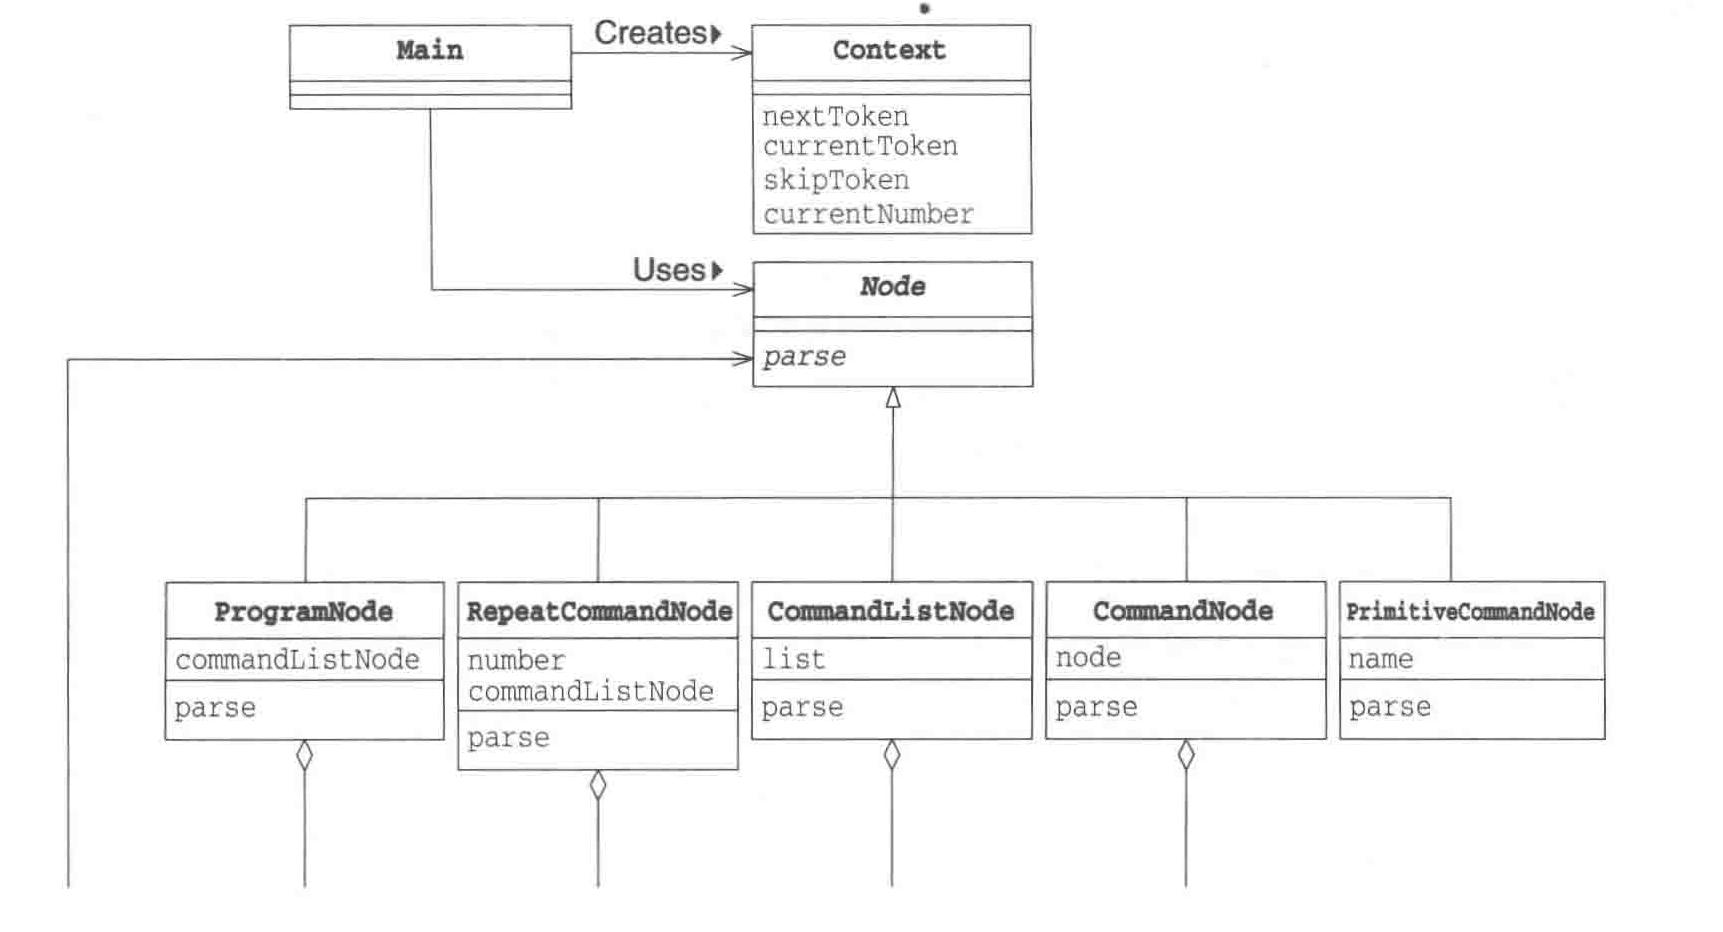
\includegraphics[width=\textwidth]{image/23-1}
	\caption{解释器模式类图}
\end{figure}
\begin{figure}[!h]
	\centering
	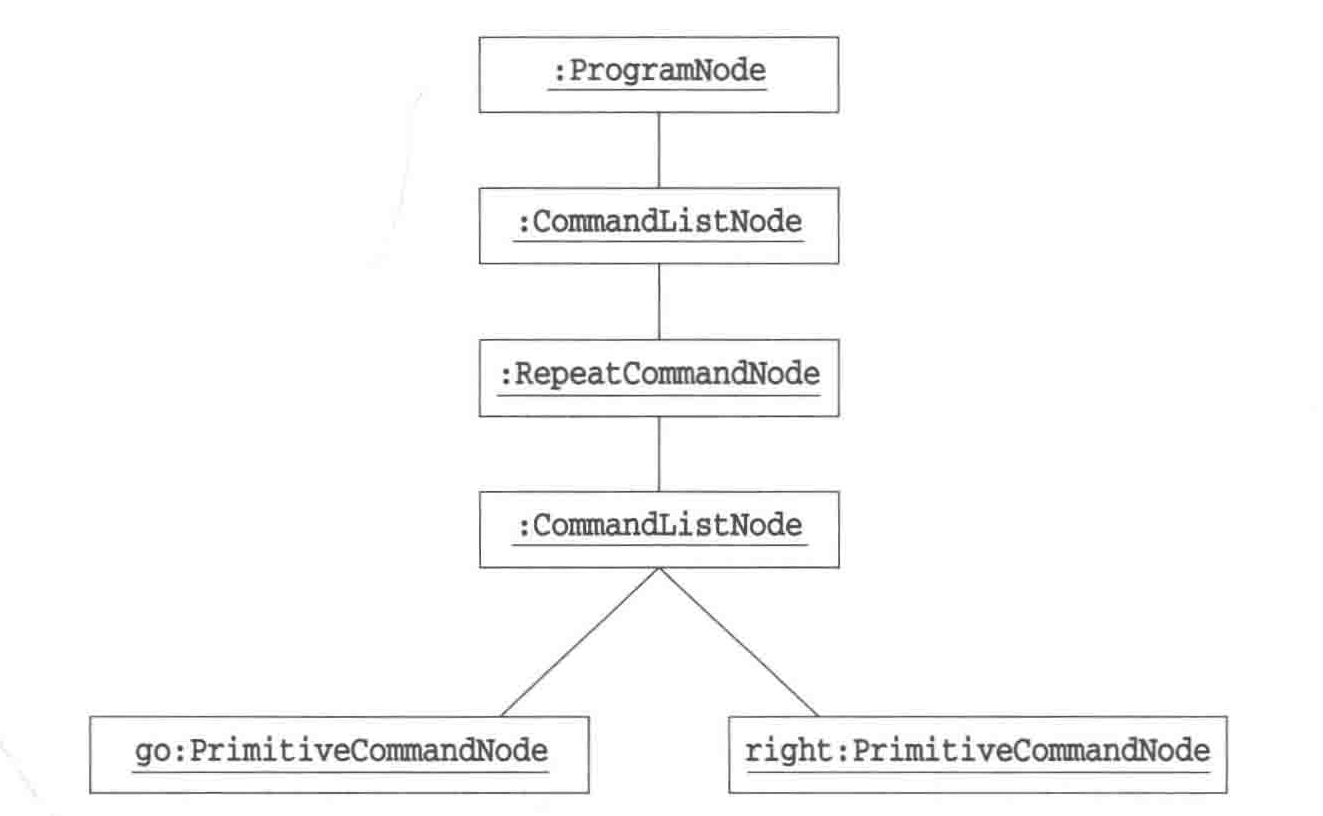
\includegraphics[width=0.8\textwidth]{image/23-2}
	\caption{语法树}
\end{figure}
\begin{lstlisting}
public abstract class Node {
	public abstract void parse(Context context) throws ParseException;
}
\end{lstlisting}
\begin{lstlisting}
// <command> ::= <repeat command> | <primitive command>
public class CommandNode extends Node {
	private Node node;
	@Override
	public void parse(Context context) throws ParseException {
		if(context.currentToken().equals("repeat")) {
			node = new RepeatCommandNode();
			node.parse(context);
		} else {
			node = new PrimitiveCommandNode();
			node.parse(context);
		}
	}
	
	public String toString() {
		return node.toString();
	}
}
\end{lstlisting}
\begin{lstlisting}
// 对应语法 <command list> ::= <command>* end
public class CommandListNode extends Node {
	private List<Node> list = new ArrayList<>();
	
	public void parse(Context context) throws ParseException {
		while (true) {
			if(context.currentToken()==null) {
				throw new ParseException("Missing 'end'", 0);
			} else if(context.currentToken().equals("end")) {
				context.skipToken("end");
				break;
				} else {
				Node commandNode = new CommandNode();
				commandNode.parse(context);
				list.add(commandNode);
			}
		}
	}
	
	public String toString() {
		return list.toString();
	}
}
\end{lstlisting}
\begin{lstlisting}
// <primitive command> ::= go | right | left
public class PrimitiveCommandNode extends Node {
	private String name;
	
	public void parse(Context context) throws ParseException {
		name = context.currentToken();
		context.skipToken(name);
		if (!name.equals("go") && !name.equals("right") && !name.equals("left")) {
			throw new ParseException(name + " is undefined",0);
		}
	}
	
	public String toString() {
		return name;
	}
}
\end{lstlisting}
\begin{lstlisting}
// 对应语法:<program> ::= program <command list>
public class ProgramNode extends Node{
	private Node commandListNode;

	public void parse(Context context) throws ParseException {
		context.skipToken("program");
		commandListNode = new CommandListNode();
		commandListNode.parse(context);
	}
	
	public String toString() {
		return "[ program " + commandListNode +']';
	}
}
\end{lstlisting}
\begin{lstlisting}
// <repeat command> ::= repeat <number> <command list>
public class RepeatCommandNode extends Node {
	private int number;
	private Node commandListNode;
	
	public void parse(Context context) throws ParseException {
		context.skipToken("repeat");
		number = context.currentNumber();
		context.nextToken();
		commandListNode = new CommandListNode();
		commandListNode.parse(context);
	}
	
	public String toString() {
		return "[repeat " + number + " " + commandListNode + "]";
	}
}
\end{lstlisting}
\begin{lstlisting}
public class Context {
	private StringTokenizer tokenizer;
	private String currentToken;
	
	public Context(String text) {
		tokenizer = new StringTokenizer(text);
		nextToken();
	}
	
	// 获取下一个标记
	public String nextToken() {
		if (tokenizer.hasMoreTokens()) {
			currentToken = tokenizer.nextToken();
		} else {
			currentToken = null;
		}
		return currentToken;
	}
	
	// 获取当前标记
	public String currentToken() {
		return currentToken;
	}
	
	//先检查当前标记,然后获取下一个标记
	public void skipToken(String token) throws ParseException {
		if (!token.equals(currentToken)) {
			throw new ParseException("Waring: " + token + " is expected, but " + currentToken + " is found", 0);
		}
		nextToken();
	}
	
	//获取当前标记对应的数值
	public int currentNumber() throws ParseException {
		int number = 0;
		try {
			number = Integer.parseInt(currentToken);
		} catch (NumberFormatException e) {
			throw new ParseException("Waring: " + e, 0);
		}
		return number;
	}
}
\end{lstlisting}
\begin{lstlisting}
public class Main {
	public static void main(String[] args) {
		try {
			BufferedReader reader = new BufferedReader(
			new FileReader("program.txt"));
			String text;
			while ((text = reader.readLine()) != null) {
				System.out.println("text = \"" + text + "\"");
				Node node = new ProgramNode();
				node.parse(new Context(text));
				System.out.println("node = " + node);
			}
			reader.close();
		} catch (Exception e) {
			e.printStackTrace();
		}
	}
}
\end{lstlisting}
\begin{lstlisting}
//output
text = "program end"
node = [ program []]
text = "program go end"
node = [ program [go]]
text = "program go right go right go right go right end"
node = [ program [go, right, go, right, go, right, go, right]]
text = "program repeat 4 go right end end"
node = [ program [[repeat 4 [go, right]]]]
text = "program repeat 4 repeat 3 go right go left end right end end"
node = [ program [[repeat 4 [[repeat 3 [go, right, go, left]], right]]]]
\end{lstlisting}
\section{解释器模式实现——例二}
\begin{figure}[!h]
	\centering
	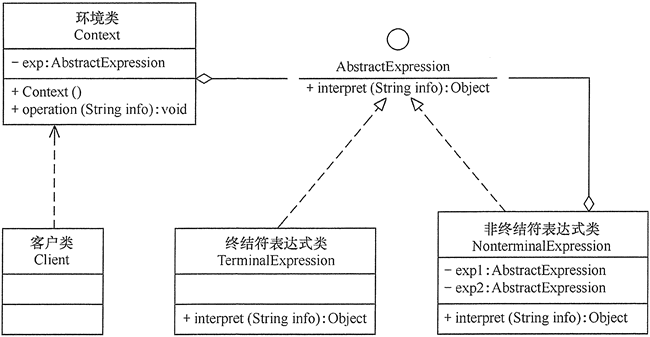
\includegraphics[width=0.8\textwidth]{image/23-3}
	\caption{解释器模式的结构图}
\end{figure}
\begin{lstlisting}
//抽象表达式类
interface AbstractExpression {
	public Object interpret(String info);    //解释方法
}
\end{lstlisting}
\begin{lstlisting}
//终结符表达式类
class TerminalExpression implements AbstractExpression {
	public Object interpret(String info) {
		//对终结符表达式的处理
	}
}
\end{lstlisting}
\begin{lstlisting}
//非终结符表达式类
class NonterminalExpression implements AbstractExpression {
	private AbstractExpression exp1;
	private AbstractExpression exp2;
	
	public Object interpret(String info) {
		//非对终结符表达式的处理
	}
}
\end{lstlisting}
\begin{lstlisting}
//环境类
public class Context {
	private AbstractExpression exp;
	
	public Context() {
		//数据初始化
	}
	
	public void operation(String info) {
		//调用相关表达式类的解释方法
	}
}
\end{lstlisting}
\section{模式扩展}
解释器模式在实际的软件开发中使用比较少,因为它会引起效率、性能以及维护等问题。如果碰到对表达式的解释,在 Java 中可以用 Expression4J 、MESP(Math Expression String Parser) 或 Jep (Java expression parser)等来设计。
\begin{lstlisting}
public class JepDemo
{
	public static void main(String[] args) throws JepException
	{
		Jep jep=new Jep();
		//定义要计算的数据表达式
		String 存款利息="本金*利率*时间";
		//给相关变量赋值
		jep.addVariable("本金",10000);
		jep.addVariable("利率",0.038);
		jep.addVariable("时间",2);
		jep.parse(存款利息);    //解析表达式
		Object accrual=jep.evaluate();    //计算
		System.out.println("存款利息:"+accrual);
	}
}
\end{lstlisting}
\section{扩展思路}
\begin{enumerate}
	\item 其他mini语言:正则表达式、检索表达式、批处理语言
	\item 注意跳过标记和读取标记。
\end{enumerate}
\section{相关设计模式}
\begin{enumerate}
	\item Composite模式:使用Composite实现NonterminalExpression角色;
	\item Flyweight模式:共享TerminalExpression角色;
	\item Visitor模式:使用Visitor访问语法树的各个节点。
\end{enumerate}